\chapter{Results}
In conclusion these are the results of our resulting models applied on the test set.
Note that the tests are made only on the model from scratch and the fine-tuned one, because the feature extraction
one underperforms in every way in comparison of the fine-tuned model. 

\section{From Scratch Model}

\begin{table}[H]
	\centering
	\begin{tabular}{|l|c|}
		\hline
		\textbf{From scratch} & \\
		\hline
		Test Loss & 0.08954 \\
		Test Accuracy & 97.59\% \\
		\hline
	\end{tabular}
    \caption{Numerical accuracy and loss}
\end{table}

\begin{table}[H]
	\centering
	\begin{tabular}{lcccc}
		\hline
		\textbf{Class} & \textbf{Precision} & \textbf{Recall} & \textbf{F1-Score} & \textbf{Support} \\
		\hline
		Strawberry\_healthy & 1.00 & 0.89 & 0.94 & 63 \\
		Tomato\_healthy & 0.93 & 1.00 & 0.96 & 62 \\
		Tomato\_Septoria\_leaf\_spot & 1.00 & 1.00 & 1.00 & 28 \\
		Cherry\_healthy & 0.98 & 0.98 & 0.98 & 165 \\
		Potato\_healthy & 0.96 & 1.00 & 0.98 & 150 \\
		Peach\_Bacterial\_spot & 1.00 & 1.00 & 1.00 & 105 \\
		Grape\_Black\_rot & 0.86 & 1.00 & 0.92 & 86 \\
		Tomato\_Tomato\_mosaic\_virus & 0.85 & 1.00 & 0.92 & 52 \\
		Tomato\_Leaf\_Mold & 1.00 & 1.00 & 1.00 & 119 \\
		Strawberry\_Leaf\_scorch & 0.99 & 0.92 & 0.95 & 99 \\
		Tomato\_Late\_blight & 1.00 & 1.00 & 1.00 & 116 \\
		Corn\_healthy & 0.94 & 1.00 & 0.97 & 118 \\
		Squash\_Powdery\_mildew & 1.00 & 0.99 & 1.00 & 139 \\
		Tomato\_Early\_blight & 0.99 & 1.00 & 1.00 & 108 \\
		Grape\_healthy & 0.98 & 0.98 & 0.98 & 43 \\
		Cherry\_Powdery\_mildew & 1.00 & 1.00 & 1.00 & 551 \\
		Pepper\_bell\_healthy & 0.99 & 0.98 & 0.99 & 230 \\
		Peach\_healthy & 0.97 & 0.97 & 0.97 & 36 \\
		Tomato\_Tomato\_Yellow\_Leaf\_Curl\_Virus & 0.94 & 0.99 & 0.97 & 100 \\
		Apple\_healthy & 0.99 & 0.99 & 0.99 & 148 \\
		Potato\_Late\_blight & 0.98 & 1.00 & 0.99 & 100 \\
		Corn\_Northern\_Leaf\_Blight & 1.00 & 0.95 & 0.97 & 100 \\
		Pepper\_bell\_Bacterial\_spot & 0.88 & 0.47 & 0.61 & 15 \\
		Grape\_Leaf\_blight & 0.97 & 0.97 & 0.97 & 37 \\
		Raspberry\_healthy & 0.98 & 0.99 & 0.99 & 509 \\
		Apple\_Cedar\_apple\_rust & 1.00 & 0.99 & 0.99 & 184 \\
		Corn\_Common\_rust & 0.99 & 1.00 & 1.00 & 111 \\
		Soybean\_healthy & 0.96 & 0.98 & 0.97 & 46 \\
		Tomato\_Bacterial\_spot & 0.98 & 0.97 & 0.97 & 213 \\
		Potato\_Early\_blight & 0.96 & 0.94 & 0.95 & 100 \\
		Grape\_Esca & 0.99 & 0.93 & 0.96 & 191 \\
		Tomato\_Target\_Spot & 0.97 & 0.99 & 0.98 & 95 \\
		Apple\_Apple\_scab & 0.99 & 0.88 & 0.93 & 177 \\
		Blueberry\_healthy & 0.93 & 1.00 & 0.96 & 159 \\
		\hline
		\textbf{Accuracy} & & & 0.98 & 5438 \\
		\textbf{Macro Avg} & 0.97 & 0.96 & 0.96 & 5438 \\
		\textbf{Weighted Avg} & 0.98 & 0.98 & 0.98 & 5438 \\
		\hline
	\end{tabular}
	\caption{Classification Report}
\end{table}

\begin{figure}[H]
    \centering
    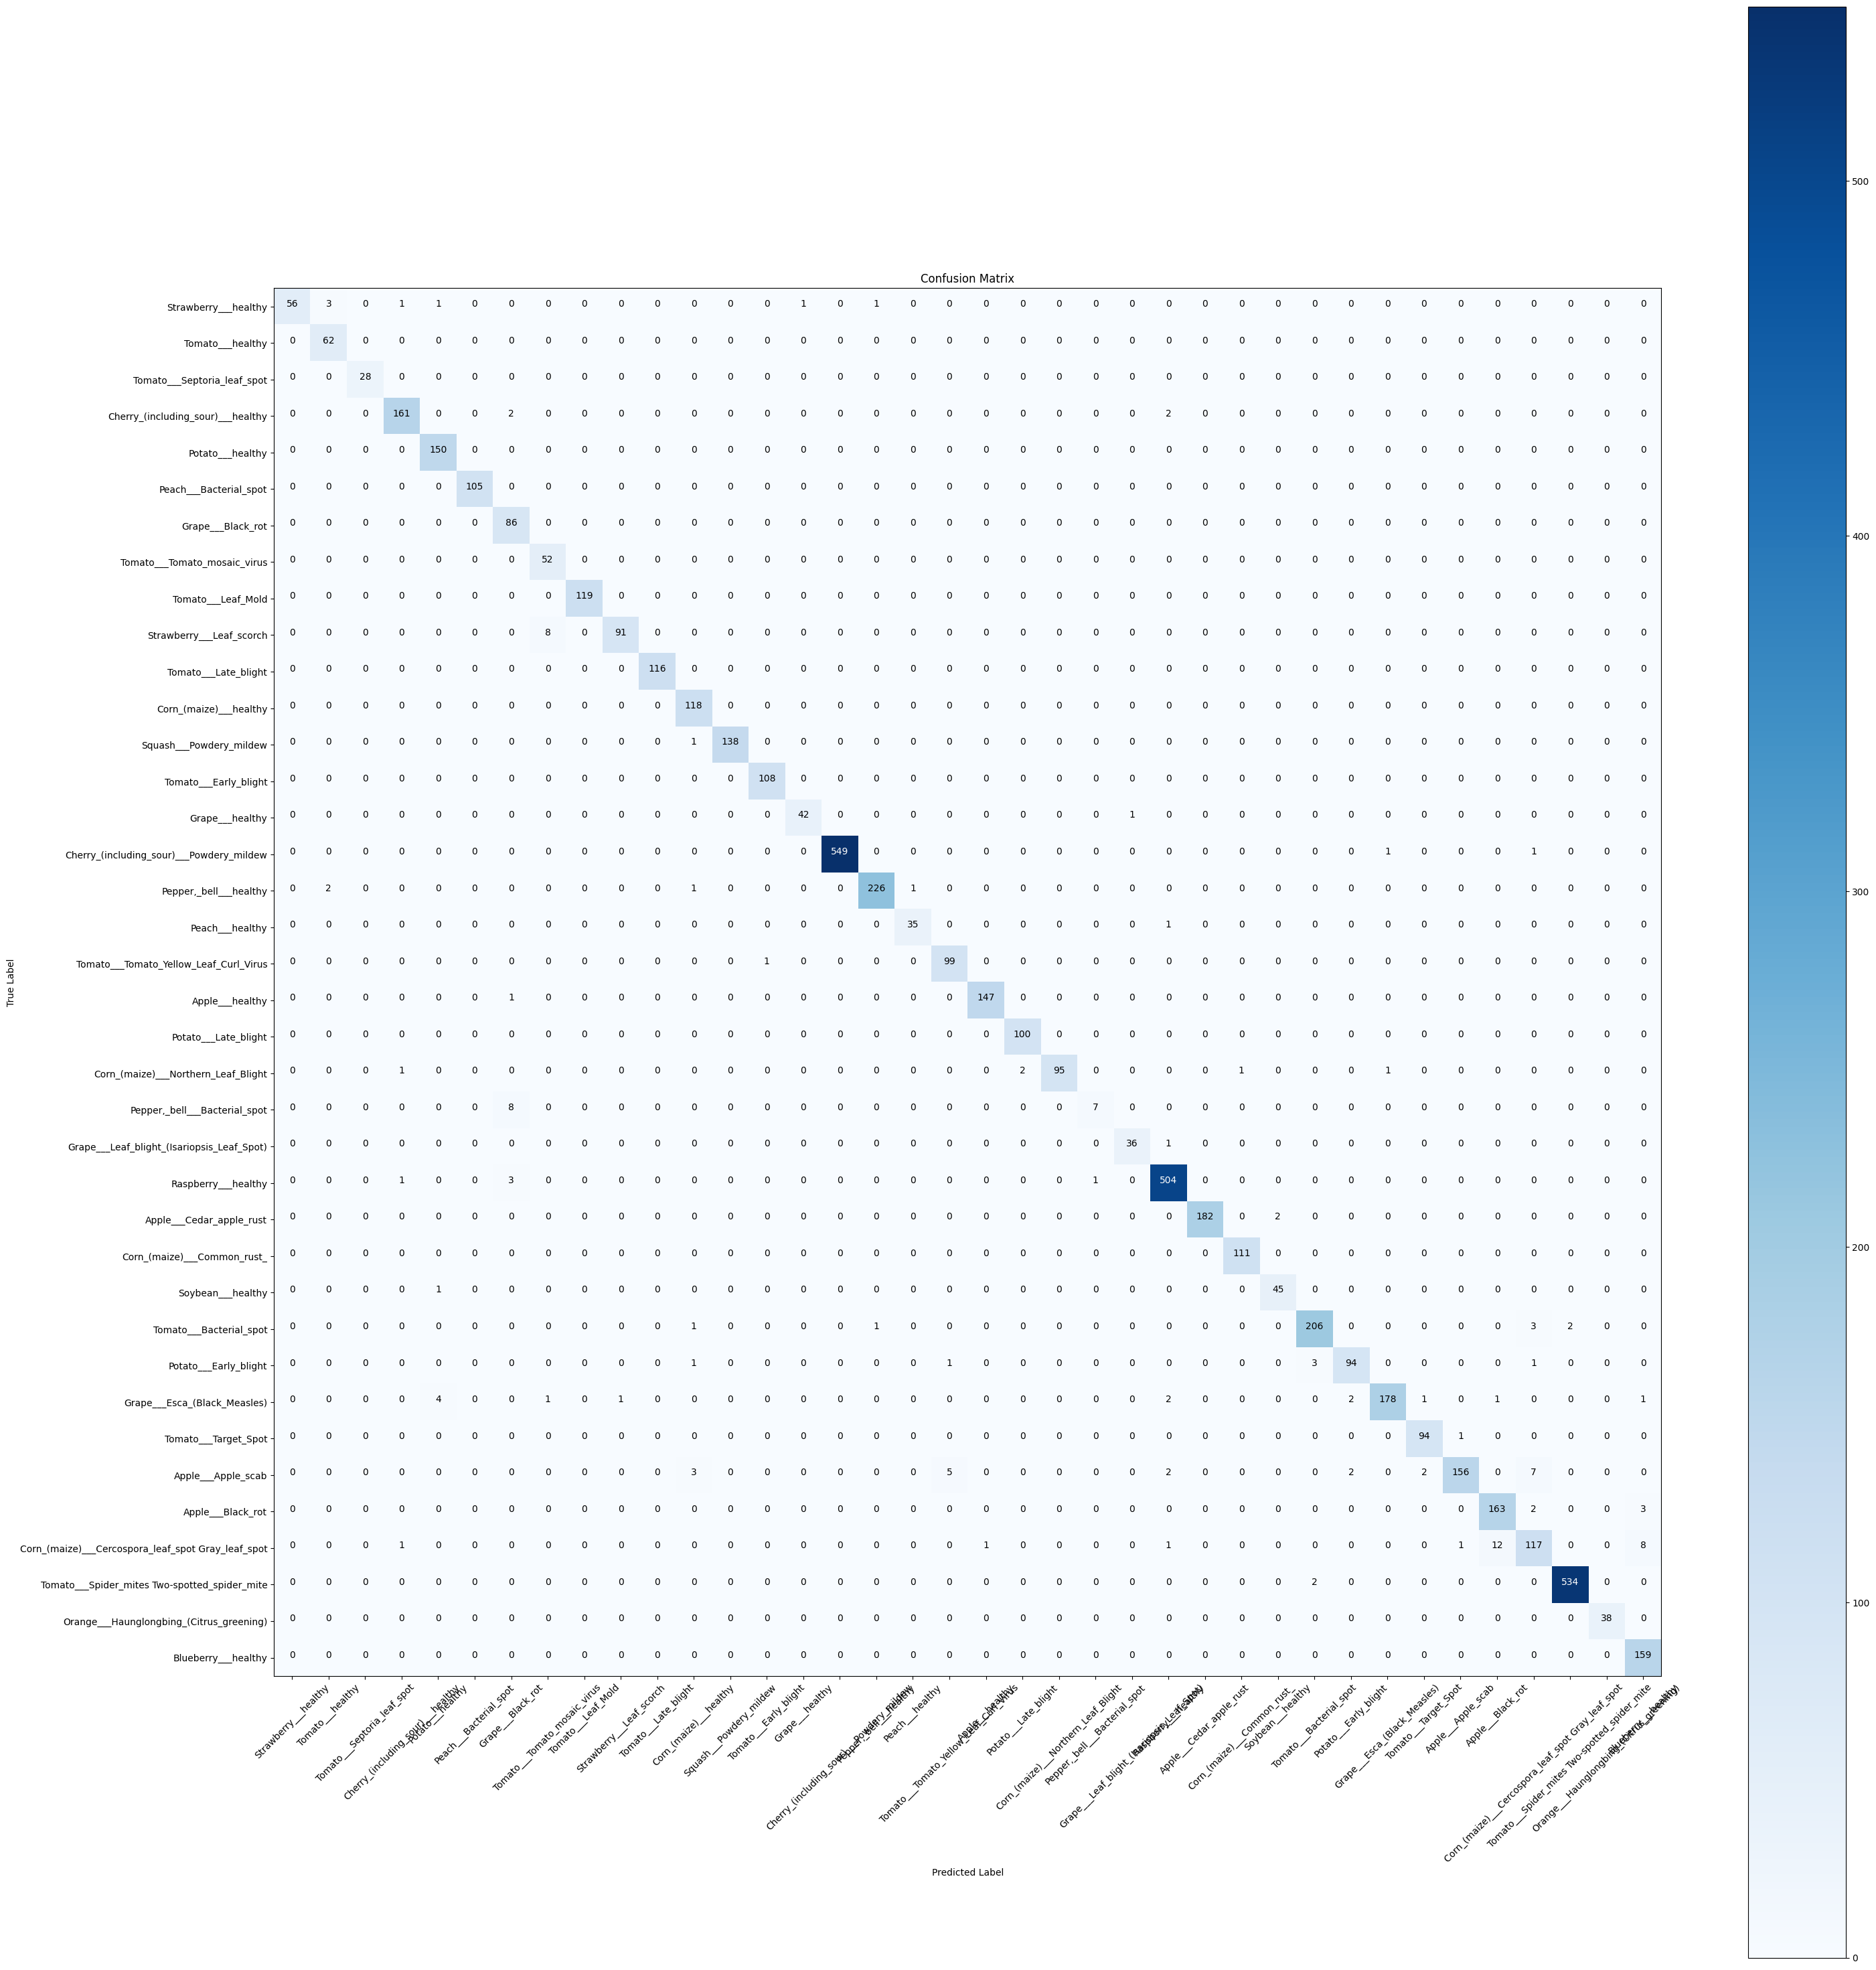
\includegraphics[width= 0.9\textwidth]{assets/FSConfMatrix.png} 
    \caption{Confusion Matrix} 
    \label{fig:immagine}
\end{figure}

Analysis of the confusion matrix and the F1-scores for individual classes reveals that the class posing the most significant
challenge is \textit{Pepper\_bell\_Bacterial\_spot}, with an F1-score of 61\% (notably, the lowest recall at 47\%). 
This issue may primarily stem from the limited availability of images for this particular class. This hypothesis 
gains support when considering that all other classes, benefiting from more extensive support, consistently 
perform at a significantly higher level, consistently exceeding a 90\% F1-score.

\section{Fine Tuned Model}

\begin{table}[H]
    \centering
    \begin{tabular}{|l|c|}
        \hline
        \textbf{Fine Tuned} & \\
        \hline
            Test Loss & 0.03156 \\
            \hline
            Test Accuracy & 99.01\% \\
            \hline
        \end{tabular}
     \caption{Numerical accuracy and loss}
\end{table}

\begin{table}[H]
	\centering
	\begin{tabular}{lcccc}
		\hline
		\textbf{Class} & \textbf{Precision} & \textbf{Recall} & \textbf{F1-Score} & \textbf{Support} \\
		\hline
		Strawberry\_healthy & 1.00 & 0.98 & 0.99 & 63 \\
		Tomato\_healthy & 1.00 & 1.00 & 1.00 & 62 \\
		Tomato\_Septoria\_leaf\_spot & 1.00 & 1.00 & 1.00 & 28 \\
		Cherry\_healthy & 1.00 & 0.99 & 1.00 & 165 \\
		Potato\_healthy & 1.00 & 1.00 & 1.00 & 150 \\
		Peach\_Bacterial\_spot & 1.00 & 1.00 & 1.00 & 105 \\
		Grape\_Black\_rot & 1.00 & 1.00 & 1.00 & 86 \\
		Tomato\_Tomato\_mosaic\_virus & 0.98 & 0.94 & 0.96 & 52 \\
		Tomato\_Leaf\_Mold & 1.00 & 1.00 & 1.00 & 119 \\
		Strawberry\_Leaf\_scorch & 0.96 & 0.99 & 0.98 & 99 \\
		Tomato\_Late\_blight & 1.00 & 1.00 & 1.00 & 116 \\
		Corn\_healthy & 1.00 & 1.00 & 1.00 & 118 \\
		Squash\_Powdery\_mildew & 1.00 & 1.00 & 1.00 & 139 \\
		Tomato\_Early\_blight & 1.00 & 1.00 & 1.00 & 108 \\
		Grape\_healthy & 1.00 & 1.00 & 1.00 & 43 \\
		Cherry\_Powdery\_mildew & 1.00 & 1.00 & 1.00 & 551 \\
		Pepper\_bell\_healthy & 0.99 & 0.98 & 0.99 & 230 \\
		Peach\_healthy & 0.88 & 1.00 & 0.94 & 36 \\
		Tomato\_Tomato\_Yellow\_Leaf\_Curl\_Virus & 1.00 & 0.99 & 0.99 & 100 \\
		Apple\_healthy & 0.99 & 1.00 & 1.00 & 148 \\
		Potato\_Late\_blight & 0.99 & 1.00 & 1.00 & 100 \\
		Corn\_Northern\_Leaf\_Blight & 1.00 & 0.94 & 0.97 & 100 \\
		Pepper\_bell\_Bacterial\_spot & 0.71 & 1.00 & 0.83 & 15 \\
		Grape\_Leaf\_blight & 1.00 & 1.00 & 1.00 & 37 \\
		Raspberry\_healthy & 1.00 & 1.00 & 1.00 & 509 \\
		Apple\_Cedar\_apple\_rust & 0.99 & 1.00 & 1.00 & 184 \\
		Corn\_Common\_rust & 1.00 & 1.00 & 1.00 & 111 \\
		Soybean\_healthy & 1.00 & 1.00 & 1.00 & 46 \\
		Tomato\_Bacterial\_spot & 1.00 & 1.00 & 1.00 & 213 \\
		Potato\_Early\_blight & 1.00 & 0.94 & 0.97 & 100 \\
		Grape\_Esca & 0.98 & 0.98 & 0.98 & 191 \\
		Tomato\_Target\_Spot & 1.00 & 0.88 & 0.94 & 95 \\
		Apple\_Apple\_scab & 0.99 & 0.98 & 0.99 & 177 \\
		Blueberry\_healthy & 0.99 & 1.00 & 0.99 & 159 \\
		\hline
		\textbf{Accuracy} & & & 0.99 & 5438 \\
		\textbf{Macro Avg} & 0.98 & 0.99 & 0.98 & 5438 \\
		\textbf{Weighted Avg} & 0.99 & 0.99 & 0.99 & 5438 \\
		\hline
	\end{tabular}
	\caption{Classification Report}
\end{table}

\begin{figure}[H]
    \centering
    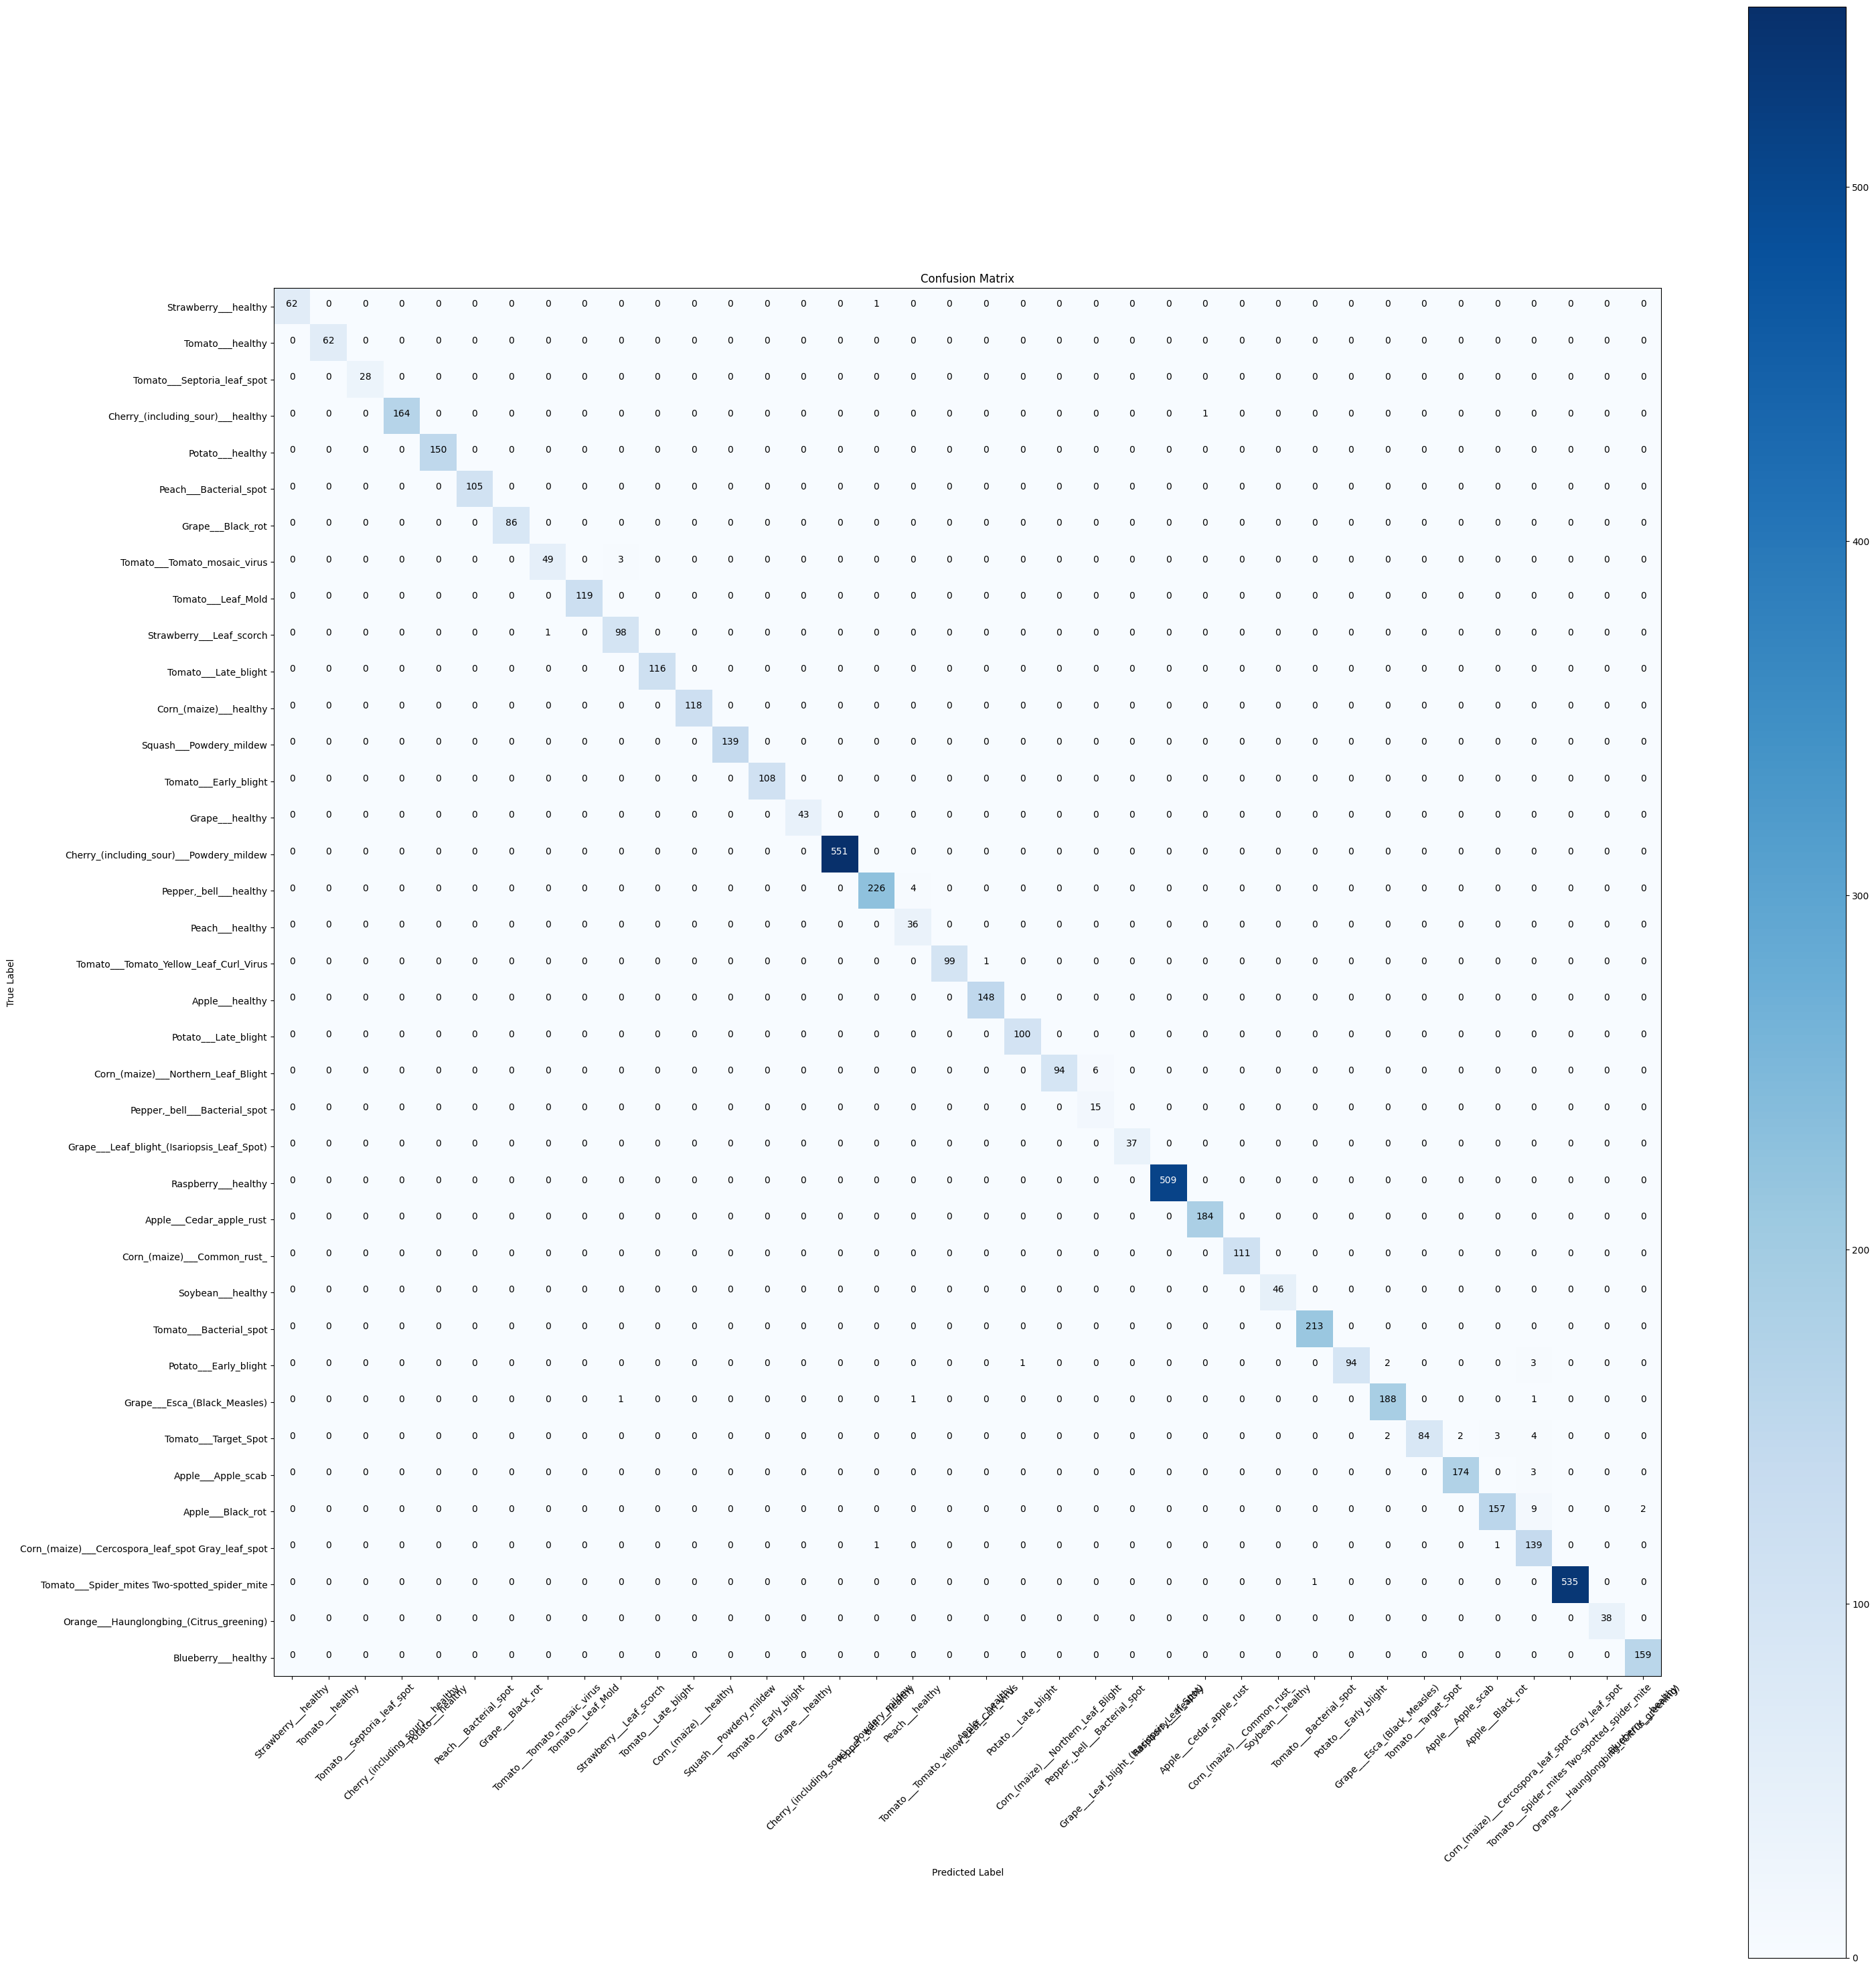
\includegraphics[width= 0.9\textwidth]{assets/FTConfMatrix.png} 
    \caption{Confusion Matrix} 
    \label{fig:immagine}
\end{figure}

Upon examination, it becomes evident that this model has surpassed its predecessor, achieving higher F1-scores and 
accuracy rates for the majority of classes. Impressively, even in the face of limited support for the 
\textit{Pepper\_bell\_Bacterial\_spot} class, the model successfully classifies it with a commendable accuracy score of 83\%.

\section{Conclusion}

In summary, our study highlights the significant advantages of fine-tuning a pre-trained model over building one from 
scratch in the leaf classification task. The fine-tuned model demonstrated exceptional performance, achieving an accuracy
of 99.01\%, which effectively categorizes leaves into multiple classes. While the from-scratch model, while lighter 
in complexity, still achieved a respectable accuracy of 97.59\%, the superior performance of the fine-tuned model 
underscores the value of leveraging pre-trained networks for image classification tasks.

It's crucial to emphasize that the 99.01\% accuracy achieved by the fine-tuned model meets the specific classification 
requirements of our study, ensuring reliable leaf categorization.

Moreover, it's worth noting that both models could have benefited from better support in the test set.

Additionally, we acknowledge that ensemble methods, although not implemented due to resource and time constraints 
in our academic setting, could have potentially further improved our classification results.

In conclusion, our findings underscore the effectiveness of fine-tuning pre-trained models and highlight the practicality 
of achieving impressive accuracy levels in leaf classification